\documentclass[10pt,twocolumn]{article}
\usepackage[a4paper,margin=0.75in,columnsep=0.25in]{geometry}
\usepackage{iftex}
\ifTUTeX
  \usepackage{fontspec} % XeTeX/Tectonic: OpenType Latin Modern keeps ligatures searchable
\else
  \usepackage[T1]{fontenc}
  \usepackage{lmodern}
\fi
\usepackage{microtype}
\usepackage{amsmath,amssymb}
\usepackage{booktabs}
\usepackage{graphicx}
\usepackage{xcolor}
\usepackage[numbers,sort&compress]{natbib}
\usepackage[hidelinks]{hyperref}
\usepackage{titlesec}
\titlespacing*{\section}{0pt}{6pt}{3pt}
\titlespacing*{\subsection}{0pt}{4pt}{2pt}
\setlength{\textfloatsep}{8pt}

\title{\vspace{-1.2em}\textbf{Where Does an Agent Go Wrong? Step-Level Confidence\\from Internal States in Multi-Step LLM Agents}\vspace{-0.4em}}
\author{Jiashu Shi\\ \small The University of Queensland}
\date{\vspace{-1.5em}}

\begin{document}
\maketitle

\begin{abstract}
LLM agents fail in the middle of a trajectory, yet most uncertainty estimates are computed once, for a final answer.
We study confidence at the level of individual agent steps. ReAct agents built on Qwen2.5-7B-Instruct and
Llama-3.1-8B-Instruct answer HotpotQA questions by searching a fixed set of paragraphs, and every step receives an
automatic correctness label. We ask three questions. (1)~Which signal best detects a wrong step? A linear probe on
mid-to-late hidden states reaches AUROC 0.835 and 0.878, ahead of sampling consistency (0.732, 0.773), verbalized
confidence (0.589, 0.701), token log-probability (0.556, 0.496) and a step-position baseline (0.693, 0.686). Before
the step is generated it reaches 0.78--0.80, although part of this early signal reflects step position. (2)~Do probes trained on single-step QA transfer to agent steps? Only from middle and upper layers: a
TriviaQA probe reaches 0.717 and 0.727 zero-shot. (3)~Are step errors coupled, and does that matter for trajectory
confidence? A Bayesian model with a previous-error term is preferred under PSIS-LOO in both models (signal ratio
1.49 and 1.73, coupling $g\approx-0.6$). Marginalising the unknown previous error repairs the severe
underconfidence of multiplied step confidences, but it is not consistently better calibrated than the last step's
confidence alone, and ranking and hand-off decisions improve only marginally.
\end{abstract}

\section{Introduction}
A multi-step agent can retrieve the wrong document, repeat a search, or commit to an answer too early, and a single
confidence score for the final answer says nothing about where things went wrong. For agents to hand control to a
person at the right moment, confidence must be estimated at each step and then aggregated over the trajectory.

Three gaps motivate this study. First, most uncertainty methods for LLMs, such as semantic entropy
\citep{kuhn2023semantic,farquhar2024detecting}, self-consistency \citep{wang2023selfconsistency} and verbalized
confidence \citep{xiong2024can}, were designed for single answers. Second, hidden-state probes predict the truth of
statements \citep{azaria2023internal,marks2023geometry}, the correctness of chain-of-thought steps
\citep{ni2026reprobe}, and the success of whole agent trajectories
\citep{mammen2026agents}, but whether a probe trained on ordinary QA transfers to agent steps is listed as an open
question \citep{lin2026uqagents}, and representation-based detectors are known to fail out of distribution
\citep{dubanowska2025representation}. Third, multiplying step-level probabilities assumes independent steps, while
step errors in agents are positively coupled \citep{lin2026uqagents}.

Our contributions are: (i)~an offline agent benchmark with automatic step labels and four step-level signals;
(ii)~evidence that hidden-state probes detect wrong steps better than output-based signals and step position, and
carry part of this signal before the step is written; (iii)~a layer-dependent picture of probe transfer from single-step QA; and (iv)~a Bayesian model
comparison, in the style of our earlier work on count time series \citep{shi2026bayesian}, showing that step errors
are coupled, and that marginalising the coupling avoids the underconfidence of multiplied step confidences, although
it is not consistently better than the last step's confidence alone.

\begin{table*}[t]
\centering\small
\caption{Step-level detection on the test split (Qwen: 902 steps, 68.5\% correct; Llama: 1028 steps, 68.2\%
correct). $\Delta$ = AUROC gap to the action-token probe with 95\% episode-bootstrap CI. Probe layers chosen on the
training split: Qwen layer 20 of 28 for all read-out points (mean pooling); Llama layer 23 of 32 (last token) for
action tokens and layer 18 for the earlier points.}
\label{tab:rq1}
\begin{tabular}{@{}lcccc@{}}
\toprule
& \multicolumn{2}{c}{Qwen2.5-7B} & \multicolumn{2}{c}{Llama-3.1-8B} \\
\cmidrule(lr){2-3}\cmidrule(l){4-5}
Signal & AUROC & $\Delta$ [95\% CI] & AUROC & $\Delta$ [95\% CI] \\
\midrule
Probe: action tokens & \textbf{0.835} & -- & \textbf{0.878} & -- \\
Probe: before action & 0.788 & $-0.046$ [$-0.072$, $-0.022$] & 0.791 & $-0.087$ [$-0.112$, $-0.063$] \\
Probe: before step & 0.778 & $-0.057$ [$-0.083$, $-0.031$] & 0.795 & $-0.084$ [$-0.110$, $-0.058$] \\
Sampling consistency & 0.732 & $-0.102$ [$-0.136$, $-0.067$] & 0.773 & $-0.105$ [$-0.140$, $-0.071$] \\
Verbalized confidence & 0.589 & $-0.247$ [$-0.298$, $-0.197$] & 0.701 & $-0.177$ [$-0.212$, $-0.143$] \\
Token log-prob (mean) & 0.556 & $-0.279$ [$-0.322$, $-0.237$] & 0.496 & $-0.383$ [$-0.421$, $-0.343$] \\
\midrule
Step index & 0.696 & $-0.139$ [$-0.171$, $-0.107$] & 0.675 & $-0.204$ [$-0.236$, $-0.172$] \\
Step index + action type & 0.693 & $-0.142$ [$-0.178$, $-0.106$] & 0.686 & $-0.193$ [$-0.228$, $-0.160$] \\
\bottomrule
\end{tabular}
\end{table*}

\section{Setup}
\textbf{Environment.} We use the distractor setting of HotpotQA \citep{yang2018hotpotqa}: each question comes with
ten paragraphs, two of which are supporting. The agent follows ReAct \citep{yao2023react} with two actions:
\texttt{Search[q]} returns the best-matching paragraph (exact title match, otherwise BM25), and \texttt{Finish[a]}
ends the episode. Episodes are capped at six steps. We sample 900 validation questions (600 train, 300 test).

\textbf{Step labels.} A \texttt{Search} is correct if it returns a supporting paragraph not retrieved before; a
\texttt{Finish} is correct if its token F1 with the gold answer is at least 0.5; unparsable actions are incorrect.
No judge model is needed. An episode succeeds if its final answer is correct.

\textbf{Signals.} For every step we record: hidden states of eight evenly spaced layers, mean-pooled over the
action tokens and at the last action token (teacher-forced); the mean and minimum token log-probability of the
action; sampling consistency, the share of five sampled alternatives ($T=0.7$) whose action is equivalent to the
greedy one (two searches are equivalent if they return the same paragraph); and verbalized confidence, a 0--100
rating from the same model in a separate prompt.

\textbf{Models.} Qwen2.5-7B-Instruct \citep{qwen2024qwen25} and Llama-3.1-8B-Instruct \citep{grattafiori2024llama3},
both in 4-bit NF4 on a single RTX 4070 Ti, with identical prompts, questions and settings. The Qwen agent takes 3.0
steps per question (2744 steps), succeeds on 60.7\% of test questions and leaves 4.7\% of test episodes unanswered;
the Llama agent takes 3.4 steps (3077 steps), succeeds on 70.0\% and leaves 10.3\% unanswered.

\begin{figure*}[t]
\centering
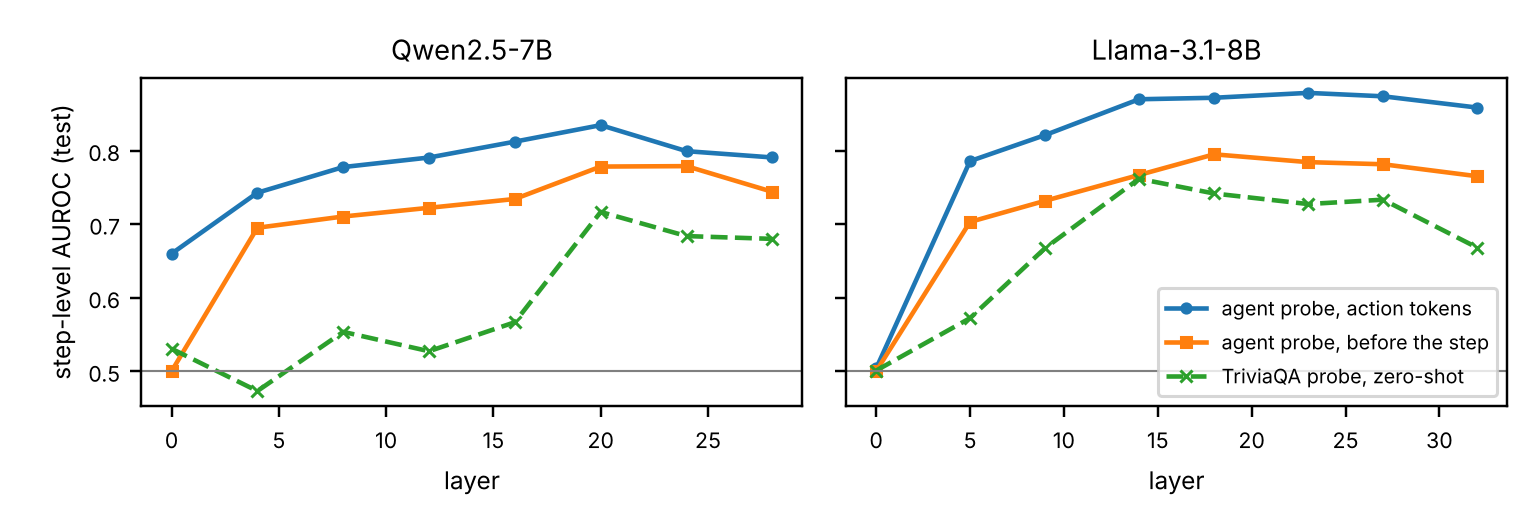
\includegraphics[width=0.8\textwidth]{figures/layers_both.png}
\vspace{-1.6em}
\caption{Test AUROC by layer: probes trained on agent steps (action tokens and before the step) and zero-shot
transfer of a TriviaQA probe. Pooling as selected per model.}
\label{fig:layers}
\end{figure*}

\section{Methods}
\textbf{Probes.} A probe is standardisation, PCA to 64 dimensions and logistic regression. Pooling and layer are
chosen by out-of-fold AUROC on the training split, with folds grouped by question. Output-based signals are mapped to
probabilities by Platt scaling \citep{platt1999probabilistic} on the training split. Position baselines are
logistic regressions on the one-hot step index, with or without the action type, fitted on the training split. Confidence intervals resample
whole test episodes (2000 replicates).

\textbf{Earlier read-out points.} Replaying each recorded trajectory, we also read the residual stream at the last
token of ``\texttt{Thought $t$:}'' (before the step) and at the last token before ``\texttt{Action $t$:}''
(after the thought, before the action).

\textbf{Transfer.} For RQ2 the model answers 2000 TriviaQA questions \citep{joshi2017triviaqa} closed-book; a probe
trained on the answer-span states is applied to agent steps zero-shot, and after Platt scaling on 50 agent steps.

\textbf{Coupled step errors.} Let $s_t$ be the out-of-fold probe logit of step $t$, $k_t$ its action type, and
$e_{t-1}=1-y_{t-1}$ an error at the previous step ($e_0=0$). We compare
\begin{align*}
\text{M0: } & \operatorname{logit} P(y_t=1) = a_{k_t} + b_{k_t} s_t,\\
\text{M1: } & \operatorname{logit} P(y_t=1) = a_{k_t} + b_{k_t} s_t + g\, e_{t-1},
\end{align*}
with $\mathcal{N}(0,2^2)$ priors, fitted in PyMC \citep{abrilpla2023pymc} and compared by PSIS-LOO
\citep{vehtari2017practical}. We report the signal ratio $\mathrm{SR}=\Delta\mathrm{ELPD}/\mathrm{SE}$
\citep{shi2026bayesian}. At test time $y_{t-1}$ is unknown, so M1's trajectory confidence marginalises it with a
two-state forward recursion, $q_0=1$, $q_t = q_{t-1}\sigma(\eta_t) + (1-q_{t-1})\sigma(\eta_t+g)$, and
$q_T$ estimates the probability that the final answer is correct. Baselines aggregate M0's step probabilities by
product, minimum, or the last step only. A hand-off policy passes an episode to a person at the first step whose
running confidence falls below $\tau$.

\section{Results}


\textbf{RQ1: hidden states detect wrong steps best.} In both models the action-token probe outperforms every
output-based signal, by at least 0.10 AUROC, and is well calibrated (ECE 0.032 and 0.026; Table~\ref{tab:rq1}). The
advantage comes from \texttt{Search} steps (Qwen 0.871 versus 0.751 for consistency; Llama 0.916 versus 0.803); on
\texttt{Finish} steps the probe is level with consistency (0.739 versus 0.699; 0.676 versus 0.692). Verbalized
confidence is compressed: 46\% (Qwen) and 51\% (Llama) of steps are rated 80. Token log-probability carries almost
no information, and for Llama's searches it is inverted (AUROC 0.378). Detection peaks about two-thirds of the way
up the network and declines slightly towards the output layer (Fig.~\ref{fig:layers}). Most of the signal is present
before the step is generated: a probe on the state before ``\texttt{Thought $t$:}'' reaches 0.778 and 0.795 from a
single forward pass. This beats five-sample consistency for Qwen (+0.045, CI [0.004, 0.088]) and matches it for
Llama (+0.022, CI [$-0.023$, 0.060]). The ranking is unchanged under a lenient label that does not penalise repeated
searches (probe versus consistency: 0.774 versus 0.692; 0.799 versus 0.732).

\textbf{Controlling for step position.} Later searches are more often repeats, so position alone predicts errors:
step index and action type reach AUROC 0.693 and 0.686. The action-token probe beats this baseline by 0.142 (CI
[0.106, 0.178]) and 0.193 (CI [0.160, 0.228]), adding position to the probe changes AUROC by at most 0.002, and
within each step index the probe keeps AUROC 0.77--0.85 (Qwen) and 0.81--0.89 (Llama). Before the action is known,
the fair baseline is step index alone; the pre-step probe adds 0.079 (CI [0.055, 0.103]) and 0.115 (CI [0.090,
0.140]) to it. Within a step index, however, the pre-step probe is roughly level with consistency (Qwen 0.66--0.72
versus 0.68--0.74; Llama 0.71--0.81 versus 0.64--0.77), and on late searches ($t\ge3$, 49--115 steps each) it is
close to chance (0.50--0.64). Part of its overall advantage over consistency is therefore positional.

\textbf{Steps within the same question.} Pooled AUROC mostly compares steps from different questions, so it may
partly reflect question difficulty \citep{esfandyari2026disentangling}. We therefore also pool, over test questions,
only the pairs of one correct and one wrong step from the same trajectory (Qwen: 134 of 300 questions have both
labels, 368 pairs; Llama: 137, 502 pairs; CIs resample questions). Probe AUROC falls by 0.07 and 0.09, but stays
above consistency and above step index (gap $+0.065$, CI [0.003, 0.125], and $+0.191$, CI [0.138, 0.245]), and keeps
0.74--0.80 after its logit is residualised on step index and action type by least squares on the training split
(Table~\ref{tab:within}). This compares different steps within one run, not repeated runs of the same question;
that comparison would need new runs.

\begin{table}[t]
\centering\small
\caption{Within-question AUROC on the test split: pairs of a correct and a wrong step from the same trajectory,
with 95\% question-bootstrap CI. Residualised: probe logit minus a least-squares fit on step index and action type.}
\label{tab:within}
\footnotesize\setlength{\tabcolsep}{3pt}
\begin{tabular}{@{}lcc@{}}
\toprule
Signal & Qwen2.5-7B & Llama-3.1-8B \\
\midrule
Probe: action tokens & 0.764 [0.704, 0.821] & 0.793 [0.748, 0.837] \\
\quad residualised & 0.736 [0.679, 0.793] & 0.795 [0.752, 0.838] \\
\quad \texttt{Search} only & 0.751 [0.661, 0.835] & 0.822 [0.774, 0.866] \\
Consistency & 0.700 [0.642, 0.752] & 0.655 [0.590, 0.717] \\
Step index ($-t$) & 0.698 [0.622, 0.773] & 0.602 [0.533, 0.665] \\
\bottomrule
\end{tabular}
\end{table}



\textbf{RQ2: transfer happens only from middle layers up.} A probe trained on closed-book TriviaQA answers (52\%
and 65\% correct) transfers to agent steps only above a model-specific depth (Fig.~\ref{fig:layers}). For Qwen it is
near chance up to layer 16 (AUROC 0.47--0.57) and reaches 0.717 at layer 20; for Llama the rise comes earlier,
staying at 0.73--0.76 from layer 14 to 27, with 0.727 at the selected layer. Raw probabilities are badly calibrated (ECE
0.471 and 0.248); Platt scaling on 50 agent steps reduces this (ECE $0.093\pm0.031$ and $0.122\pm0.034$) without
changing the ranking. For Qwen this matches an in-domain probe trained on the same 50 steps (AUROC
$0.731\pm0.043$); for Llama the small in-domain probe is better ($0.779\pm0.031$). Transfer is therefore partial
and layer-dependent, rather than absent as reported for broad hallucination detectors
\citep{dubanowska2025representation}.

\begin{table}[t]
\centering\small
\caption{Trajectory confidence on finished test episodes (Qwen: 286, 63.6\% correct; Llama: 269, 78.1\% correct).}
\label{tab:rq3}
\setlength{\tabcolsep}{5pt}
\begin{tabular}{@{}lcccc@{}}
\toprule
& \multicolumn{2}{c}{Qwen2.5-7B} & \multicolumn{2}{c}{Llama-3.1-8B} \\
\cmidrule(lr){2-3}\cmidrule(l){4-5}
Aggregation & AUROC & ECE & AUROC & ECE \\
\midrule
M1 forward & 0.735 & \textbf{0.027} & 0.682 & 0.104 \\
M0 last step & 0.739 & 0.057 & 0.676 & \textbf{0.096} \\
M0 minimum & 0.702 & 0.082 & 0.659 & 0.206 \\
M0 product & 0.664 & 0.200 & 0.642 & 0.326 \\
\bottomrule
\end{tabular}
\end{table}

\textbf{RQ3: step errors are coupled, but modelling it adds little over the last step.} M1 is preferred to M0 in both models
(Qwen: $\Delta$ELPD $=5.58$, SE $=3.75$, SR $=1.49$, all Pareto $k<0.16$; Llama: $\Delta$ELPD $=7.22$, SE $=4.17$,
SR $=1.73$, maximum Pareto $k=0.76$, above the 0.7 threshold beyond which PSIS-LOO is unreliable for those steps, so
the Llama comparison should be read with caution). The coupling coefficients agree closely:
$g=-0.58$ $[-0.84,-0.33]$ and $g=-0.62$ $[-0.87,-0.37]$ (90\% intervals). After an error, the odds that the next step
is correct fall to about 0.55 of their value, even given the probe signal. We read this as moderate, replicated
evidence. Multiplying step confidences badly underestimates success (mean confidence 0.44 and 0.45 versus 63.6\%
and 78.1\% observed), because a wasted search is often recovered. The forward recursion removes most of this error
(ECE gap to the product 0.142, CI [0.082, 0.186], and 0.218, CI [0.189, 0.244]; Table~\ref{tab:rq3}). Its
calibration, however, does not differ significantly from the last step alone (ECE gap last $-$ forward: CI
[$-0.030$, 0.055] and [$-0.024$, 0.033]), and in neither model does it rank episodes better than the last step (AUROC gap $-0.004$, CI [$-0.017$, 0.009]; $+0.006$, CI [$-0.015$, 0.028]). The hand-off
curve of M1 lies at or above that of M0 (Fig.~\ref{fig:handoff}), but the difference in area is not significant
(0.019, CI [$-0.003$, 0.041]; 0.005, CI [$-0.010$, 0.020]). Hand-offs typically occur at steps 2--3.

\begin{figure}[t]
\centering
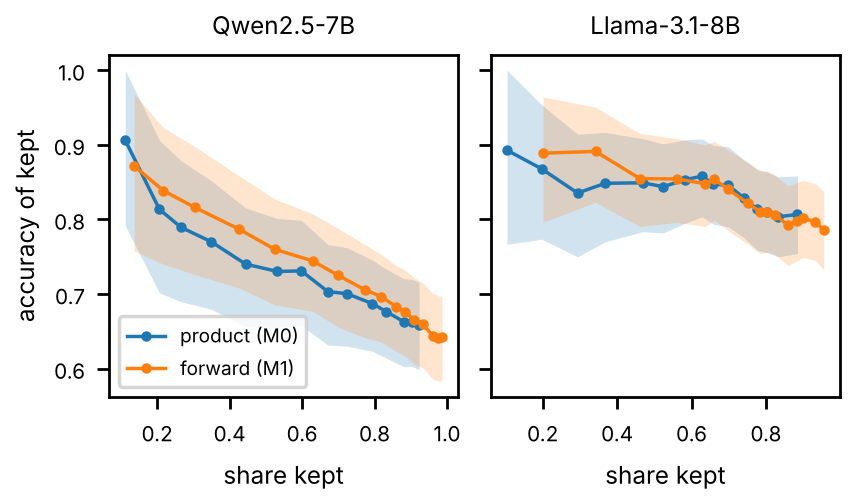
\includegraphics[width=\columnwidth]{figures/handoff_both.png}
\vspace{-1.2em}
\caption{Hand-off curves with 95\% episode-bootstrap bands. Points keeping under 10\% of episodes are omitted.}
\label{fig:handoff}
\end{figure}

\section{Discussion and Limitations}
Internal states carry information about step correctness that output-based signals and step position miss. Some
of it is available before the agent acts, beyond what step position gives, which suggests that cheap pre-emptive
hand-off is feasible; within a step index, however, the pre-step probe is only level with sampling consistency. The two models differ in how well they
verbalize confidence and in how many steps they take, yet the probe advantage, the layer profile and the size of the
error coupling are close across them. The layer profile, peaking about two-thirds of the way up and shared across
read-out points and, for transfer, across tasks, suggests a reusable representation of ``this is going well'' that
deserves mechanistic study. The probe's advantage is concentrated on retrieval steps; judging a final answer
remains as hard for the probe as for sampling. One hypothesis is that the pre-step state already encodes
whether the previous retrieval helped, which would connect the early-detection result to the coupling found in RQ3.

The study has clear limits. It uses one task, one seed and two 7--8B models in 4-bit precision. Each test split has
fewer than 300 finished trajectories, so differences between hand-off policies are within noise. Trajectory-level
results use finished episodes only; the excluded unfinished episodes (4.7\% and 10.3\% of the test split) are all
failures, so kept accuracy in the hand-off curves is optimistic. Step labels are automatic and
conservative. Features are extracted from recorded trajectories; we have not yet triggered hand-offs online.
Future work: online intervention with pre-step probes, longer-horizon environments, and trajectory-level
calibration with guarantees under history dependence.

\paragraph{Reproducibility} Code, configuration and per-step results are available at \url{https://github.com/JIASHU-S/agent-step-confidence}.

\small
\bibliographystyle{unsrtnat}
\bibliography{refs}
\end{document}
